\documentclass[border=10pt]{standalone}

\usepackage{tikz}
\usepackage{tikzsymbols}
\usetikzlibrary{calc,patterns,shapes.geometric}

\def\centerarc[#1](#2)(#3:#4:#5){\draw[#1] ($(#2)+({#5*cos(#3)},{#5*sin(#3)})$) arc (#3:#4:#5);}

\begin{document}
	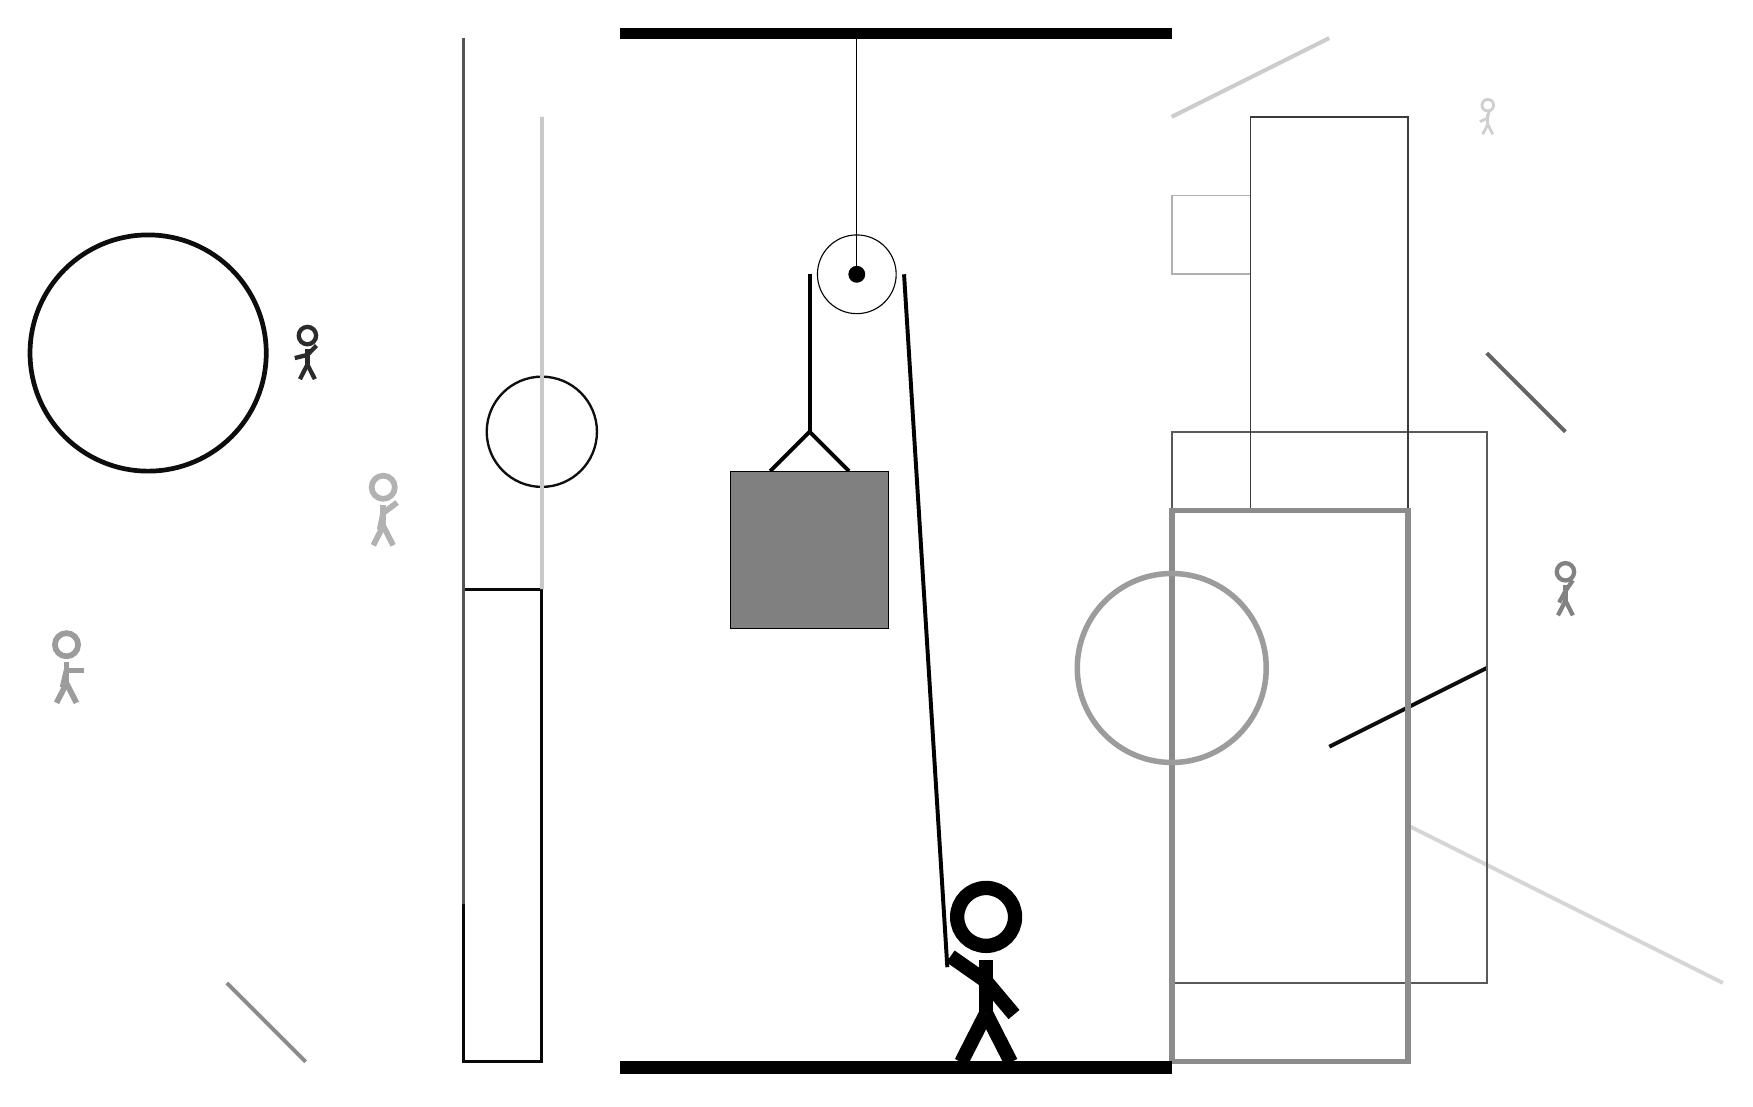
\begin{tikzpicture}
		%%%%% START %%%%%
		
		\draw[fill=black] (-2, 10) rectangle (5, 10.125);
		
		\draw (1, 7) circle (0.5);
		\draw[fill=black] (1, 7) circle (0.1);
		\draw (1, 10) -- (1, 7);
		
		\draw[line width=0.5mm] (-0.1, 4.5) -- (0.4, 5.0) -- (0.9, 4.5);
		\draw[fill=black!50] (-0.6, 4.5) rectangle (1.4, 2.5);
		
		\draw[line width=0.5mm] (0.4, 7) -- (0.4, 5.0);
		\centerarc[line width=0.5mm](1, 7)(0:180:0.6);
		\draw[line width=0.5mm](1.6, 7) -- (2.15, -1.8);
		
		\node at (2.6, -1.9) {\Strichmaxerl[10][-35][-50]};
		
		\draw[line width=0.4mm, color=black!97] (-3, 3) rectangle (-4, -3);
		
		\node[line width=0.3mm, color=black!19] at (9, 9) {\Strichmaxerl[2][24][81]};
		\draw[line width=0.5mm, color=black!95](9, 2) -- (7, 1);
		\draw[line width=0.5mm, color=black!61](10, 5) -- (9, 6);
		
		\node[line width=0.3mm, color=black!49] at (10, 3) {\Strichmaxerl[3][61][56]};
		
		\draw[line width=0.5mm, color=black!20](5, 9) -- (7, 10);
		\draw[line width=0.5mm, color=black!16](8, 0) -- (12, -2);
		\draw[line width=0.2mm, color=black!31] (6, 8) rectangle (5, 7);
		\node[line width=0.2mm, color=black!83] at (-6, 6) {\Strichmaxerl[3][14][46]};
		\node[line width=0.5mm, color=black!39] at (-9, 2) {\Strichmaxerl[4][77][0]};
		
		\draw[line width=0.4mm, color=black!67] (-4, -1) rectangle (-4, 10);
		
		\draw[line width=0.2mm, color=black!65] (5, 5) rectangle (9, -2);
		\draw [line width=0.3mm, color=black!94](-3, 5) circle (0.7);
		
		\draw[line width=0.5mm, color=black!21] (-3, 9) rectangle (-3, 3);
		\draw [line width=0.6mm, color=black!95](-8, 6) circle (1.5);
		\draw[line width=0.2mm, color=black!77] (6, 9) rectangle (8, 4);
		
		\draw[line width=0.7mm, color=black!45] (5, 4) rectangle (8, -3);
		
		\draw[line width=0.5mm, color=black!46](-7, -2) -- (-6, -3);
		\draw [line width=0.6mm, color=black!39](5, 8) circle (0.0);
		\draw [line width=0.7mm, color=black!39](5, 2) circle (1.2);
		\node[line width=0.6mm, color=black!30] at (-5, 4) {\Strichmaxerl[4][78][37]};
		
		\draw[fill=black] (-2, -3) rectangle (5, -3.15);
		
		%%%%% END %%%%%
	\end{tikzpicture}
\end{document}